\documentclass[11pt,paper=a4]{article}

%\documentclass[12pt,preprint]{aastex}


\usepackage{amsmath}
\usepackage{natbib}
\usepackage{graphicx}
\usepackage[usenames,dvipsnames]{color}
\usepackage[absolute,overlay]{textpos}
\usepackage{color}
\usepackage{multirow}

\usepackage{hyperref}
\hypersetup{
        colorlinks = true,
        linkcolor = blue,
        anchorcolor = red,
        citecolor = blue,
        filecolor = red,
        urlcolor = red
} 

\newcommand{\eht}{\overline}    
\newcommand{\fht}{\widetilde}        
\newcommand{\dr}{\frac{\partial}{\partial r}}
\newcommand{\dt}{\frac{\partial}{\partial t}}
\newcommand{\dth}{\frac{\partial}{\partial \theta}}
\newcommand{\dph}{\frac{\partial}{\partial \phi}}

\def\ef#1{#1'}
\def\ff#1{#1''}
\def\fhtc#1{\left\{#1\right\}}
\def\erho{\eht{\rho}}

% From Maxime's paper


\newcommand{\vdag}{(v)^\dagger}
\newcommand{\Teff}{T_\mathrm{eff}}
\newcommand{\Rsun}{R_\odot}
\newcommand{\dV}{\mathrm{d}V}
%\newcommand\av[1]{\overline{<#1>}}
%\newcommand\av[1]{<\overline{#1}>}


%\newcommand\av[1]{\overline{\langle{#1}\rangle}}
\def\av#1{\overline{#1}}
%\newcommand\fav[1]{\widetilde{\langle #1 \rangle}}
\def\fav#1{\widetilde{#1}}
\newcommand\br[1]{\langle #1\rangle}
\newcommand\hpartial[1]{\hat{\partial} #1}





%----------  Own Macros  --------------------------------------
\def\etal{{\it et al. }}
\def\ie{{\it i.e. }}
\def\eg{{\it e.g. }}
\def\ms{\, {M_{\odot}}}

\def\la{\hbox{\raise.5ex\hbox{$<$} 
    \kern-1.1em\lower.5ex\hbox{$\sim$}}} 
\def\ga{\hbox{\raise.5ex\hbox{$>$} 
    \kern-1.1em\lower.5ex\hbox{$\sim$}}} 
\def\msun{$M_\odot$} 

\newcommand{\SubItem}[1]{
    {\setlength\itemindent{15pt} \item[-] #1}
}



\newcommand{\mean}[1]{\ensuremath{\overline{#1}}}
\newcommand{\dgr}{\mbox{$^\circ$}}           % degrees 
\newcommand{\Msun}{\mbox{M$_\odot$\,}}         % M_sun 
\newcommand{\Lsun}{\mbox{$L_\odot$}}         % L_sun 
\newcommand{\dTdp}{\mbox{$\nabla$}}          % Temp.grad. 
\newcommand{\dTdpad}{\mbox{$\dTdp_{ad}$}}    % ad. Temp.grad. 
\newcommand{\Tmax}{\mbox{$T_{max}$}}         % T_max 
\newcommand{\Tmaxq}{\mbox{$\overline T_{max}$}} % T_max quer 
\newcommand{\RTmax}{\mbox{$R_{max}$}}        % RT_max 
\newcommand{\sTmax}{\mbox{$\sigma_T$}}       % sigma T_max 
\newcommand{\DTmax}{\mbox{$\Delta_T$}}       % Delta T_max 
\newcommand{\vexp}{\mbox{$v_{exp}^{(a)}$}}   % vexp 
\newcommand{\vprop}{\mbox{$v_{prop}^{(i)}$}} % vprop 
\newcommand{\Drinv}{\mbox{$d_{inv}$}}        % Drinv 
\newcommand{\DRinv}{\mbox{$\Delta R_{inv}$}} % DRinv 
\newcommand{\aP}{${}^\star$}                 % prime 
\newcommand{\ad}{\mbox{d}}                   % d 
\newcommand{\gsim}{\gtrsim}                  % greater sim 
\newcommand{\cm}{\mbox{\ cm}}                % units 
\newcommand{\g}{\mbox{\ g}}                  % units 
\newcommand{\s}{\mbox{\ s}}                  % units 
\newcommand{\K}{\mbox{\ K}}                  % units 
\newcommand{\erg}{\mbox{\ erg }}              % units 
\newcommand{\cms}{\mbox{\ cm s${}^{-1}$}}    % units 
\newcommand{\cmss}{\mbox{\ cm s${}^{-2}$}}    % units 
\newcommand{\Ks}{\mbox{\ K s${}^{-1}$}}    % un
\newcommand{\Kcm}{\mbox{\ K cm${}^{-1}$}}    % un
\newcommand{\mes}{\mbox{\ m s${}^{-1}$}}    % units 
\newcommand{\ergK}{\mbox{\ erg K${}^{-1}$}}    % units 
\newcommand{\gcm}{\mbox{\ g cm${}^{-3}$}}    % units 
\newcommand{\gcms}{\mbox{$\g\cm^{-1}\s^{-1}$}}    % units 
\newcommand{\ergcms}{\mbox{$\erg\cm^{-3}\s^{-1}$}}  % units 
\newcommand{\erggs}{\mbox{$\erg\g^{-1}\s^{-1}$}}  % units 
\newcommand{\ergs}{\mbox{$\erg\s^{-1}$}}  % units
\newcommand{\ergcmsK}{\mbox{$\erg\K^{-1}\cm^{-1}\s^{-1}$}}   % units 
\newcommand{\dyncm}{\mbox{\ dyn$\cm^{-2}$}}  % units 
\newcommand{\radcm}{\mbox{\ rad$^2 \cm^{-2}$\,}}  % units 
\newcommand{\radss}{\mbox{\ rad$^2 \s^{-2}$\,}}  % units 
\newcommand{\vrad}{\mbox{v$_{r}$}} 
\newcommand{\sv}{\langle\sigma v\rangle}
\newcommand{\cer}{\color{red}}
\def\eSGS{\eta_{SGS}} 

 
%  input: Math. f"ur Hydroformeln 
\newcommand{\dz}{\partial_t} 
%\newcommand{\dr}{\partial_r} 
%\newcommand{\dt}{\partial_\theta} 
\newcommand{\df}{\partial_\phi} % \dp macht in LaTeX Schwierigkeiten 
\newcommand{\ddz}{\frac{\partial}{\dz}} 
\newcommand{\ddr}{\frac{\partial}{\dr}} 
\newcommand{\ddt}{\frac{\partial}{\dt}} 
\newcommand{\ddf}{\frac{\partial}{\df}} 
%\newcommand{\vr}{v_r} 
\newcommand{\vt}{v_\theta} 
\newcommand{\vp}{v_\phi} 
\newcommand{\st}{{\,\sin\!\theta}} 
\newcommand{\ct}{{\,\cos\!\theta}} 
\newcommand{\stq}{{\,\sin^2\!\theta}} 
\newcommand{\rez}[1]{\frac{1}{#1}} 
\newcommand{\rezr}{\rez{r}} 
\newcommand{\rezrs}{\rez{r\st}} 
\newcommand\bba{\,\,\Bigl[\,\,} 
\newcommand\bbz{\,\,\Bigr]\,\,} 
\newcommand{\mbf}[1]{\mbox{\boldmath$#1$}} % bold in mmode 

\DeclareMathAlphabet{\mathpzc}{OT1}{pzc}{m}{it}

\def\todo#1{{\color{red}[#1]}}

\usepackage{titling}
\newcommand{\subtitle}[1]{%
  \posttitle{%
    \par\end{center}
    \begin{center}\large#1\end{center}
    \vskip0.5em}%
}

%\title{... title ...}
\title{Towards Complex Understanding of Turbulent Convection in Stellar Interiors Using ransX Analysis Framework}
\subtitle{Proposal For Post-Doctoctoral Research Position}

\author{Dr. Miroslav Moc\'ak}

\begin{document}

\maketitle
\bibliographystyle{plainnat}

\section{Introduction}

Contemporary ground- and space-based telescopes provide us precise stellar data leading to challenging questions and forcing us to reconsider our basic assumptions regarding turbulent convection and mixing in stars. Properties of supernova explosions studied by HST or Keck can not be linked to their progenitors conclusively \citep{Smartt2009}. Such progenitors are known to have a structure interleaved by turbulent convection shells \citep{HirschiMeynet2004}. VLT is observing massive stars with unexplained chemical peculiarities, where rotational mixing was considered to be enough to explain observations \citep{Evans2008}. Kepler spacecraft finds unexplained pulsations of $\delta$ Scuti and $\gamma$ Doradus stars \citep{UytterhoevenArxiv2011}, which depend heavily on properties of sub-surface stellar convection \citep{GuzikKaye2000}. Explanation of observed element abundances in AGB stars requires physically motivated but still inconclusive tuning for mixing between turbulent envelope convection and underlying hydrogen-free core \citep{Herwig2005}.

Turbulence is during stellar evolution one of the most fundamental processes and before taking into account binarity, magnetism or rotation of a star to explain observations, we should understand stellar turbulence well first. It is arguably the greatest weakness in the modern theory of stellar evolution, which is mostly derived from one-dimensional calculations approximating dynamic turbulent processes by simplified theories \citep{KipWeigert1990,CoxGiuli2008}. In reality, turbulent flows are multidimensional and driven by non-linear terms of the hydrodynamic Navier-Stokes equations. 

\section{Aims}

I will analyze three-dimensional (3D) hydrodynamic simulations of stellar convection within the context of Reynolds-Averaged Navier Stokes (RANS) approach pursued by \citet{Besnard1992,Livescu2009,Schwarzkopf2011}. It is a unique way of learning about turbulence based on budget analysis of hydrodynamic equations averaged in space and time, by which complexity of every term is reduced to a one-dimensional mean field.

Using this methodology, we derived RANS evolution equations for transport/flux/variance of mass, momenta, kinetic/internal/total energy, temperature, enthalpy, pressure and composition densities (no magnetic fields, no rotation) \citep{Mocak2014} and implemented them to analysis framework, that we call rans(eXtreme) or ransX\footnote{ransX is free for download and test on \href{https://github.com/mmicromegas/ransX}{https://github.com/mmicromegas/ransX}} for short. It should be noted here, that it is only one of many possible sets of equations relevant to closure problems in turbulence and there are many other formulations, which then need to approximate different terms \citep{Canuto1992,Canuto1993,CanutoHoward2001,Hanjalic2002,Alfonsi2009,Garaud2010,Canuto2011a,BiferaleMantovani2011}. 

RANS approach introduces into the averaged equations many correlations of various thermodynamic fluctuations which are essentially new unknown variables. Hence, to solve them, we need either to design appropriate closures or derive and close evolution equations for them. Either of the tasks is difficult, because stellar turbulence is anisotropic, compressible and embedded in highly stratified environment where external forces like gravity and mean background flow play an important role. But we hope that this approach could in the future allow us to study stellar evolution using solution of the mean fields hydrodynamic equations, move away from canonical form of stellar structure equations and most importantly allow for a comprehensive synergy between engineering turbulence modeling and stellar astrophysics. 

My aims encompass the following targets (their content partially overlap with each other and the estimated time of completion is stated in brackets):

\begin{itemize}  
\item publish our RANS mean-field equations implemented within ransX framework \citep{Mocak2014}\footnote{More up-to-date equation content of the ransX framework can be found here \href{https://github.com/mmicromegas/ransX/blob/master/DOCS/ransXtheoryGuide.pdf}{https://github.com/mmicromegas/ransX/blob/master/DOCS/ransXtheoryGuide.pdf}} in high-impact referred journal and validate them with new high-resolution 3D hydrodynamic simulations (2+ year)
\item help to implement the ransX framework to all hydrodynamic codes capable of simulating stellar core and envelope convection (e.g. MUSIC \citep{VialletBaraffe2011}, PROMETHEUS \citep{Fryxell1991,Mueller1991})  or stellar atmospheres in 3D and make it an analysis standard (3+ years)
\end{itemize}

%The new hydrodynamic stellar structure equations for stellar turbulence are listed below as equations (1),(2),(3),(4),(5),(6). They appear to work well (Fig.\ref{hsse:eq_simp}) but the first four equations still lack a theory that explains them and the last equation (5) requires a proper model for transport of composition density ($\nabla_r f_\alpha$) commonly treated in stars as difussion.

%\begin{align}
%\partial_r \eht{m} = & \ -\eht{\rho} \ \eht{m} \ \eht{g}_r / \Gamma_1 \eht{P} + 4 \pi r^2 \eht{\rho} &  \\
%\partial_r \eht{P} = & \ -\eht{\rho} \ \eht{g}_r \\
%\partial_r \fht{L} = & \ -4 \pi r^2 \eht{\rho} \ \eht{g}_r / \Gamma_1 + \widetilde{\epsilon}_{t} \partial_r 4 \pi r^2 \eht{\rho} \fht{u}_r  \\
%\partial_r \eht{T} = & -(\Gamma_3 -1) \ \eht{\rho} \ \eht{T} \ \eht{g}_r / \Gamma_1 \eht{P} \\
%\partial_t \fht{X}_i = & \ \fht{\dot{X}}_i^{nuc} - (1/\eht{\rho})\nabla_r f_i - \fht{u}_r \partial_r \fht{X}_i \\
%\fht{u}_r = & \ \dot{\overline{M}} / 4 \pi r^2 \overline{\rho}
%\end{align}


%\begin{figure}[!h]
%\centerline{
%  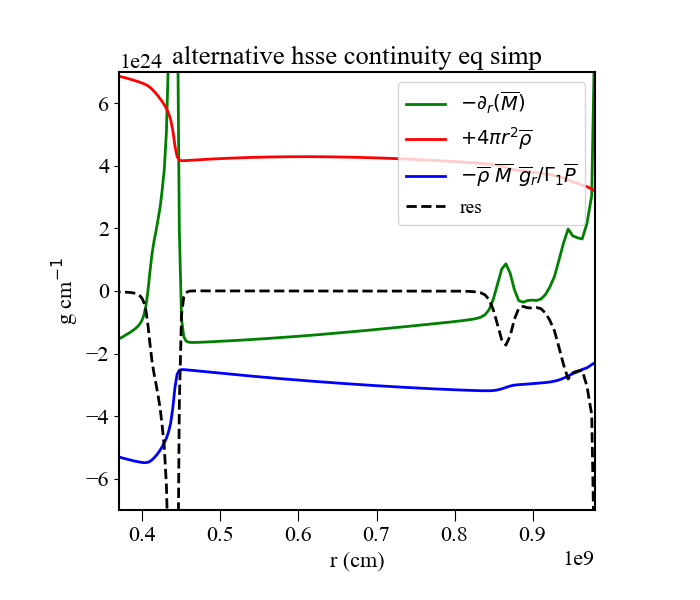
\includegraphics[width=6.3cm]{oblrez_hsse_continuity_eq_alternative_simplified.eps}
%  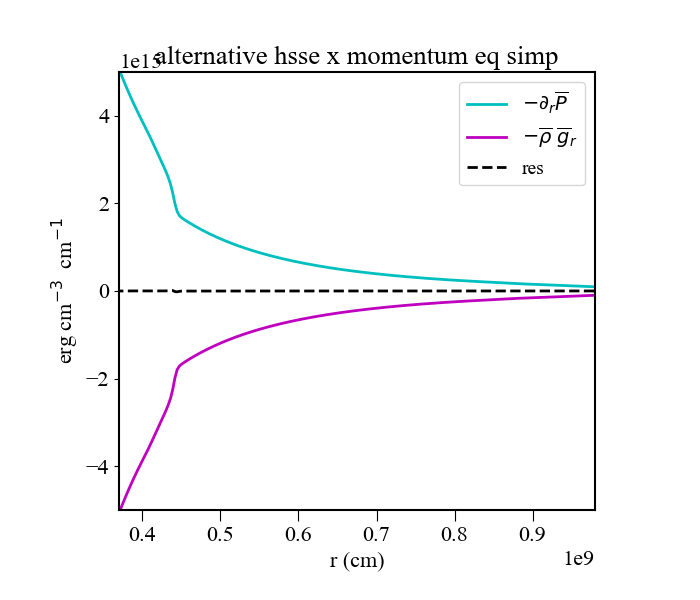
\includegraphics[width=6.3cm]{oblrez_hsse_momentum_x_eq_alternative_simplified.eps}}

%\centerline{
%  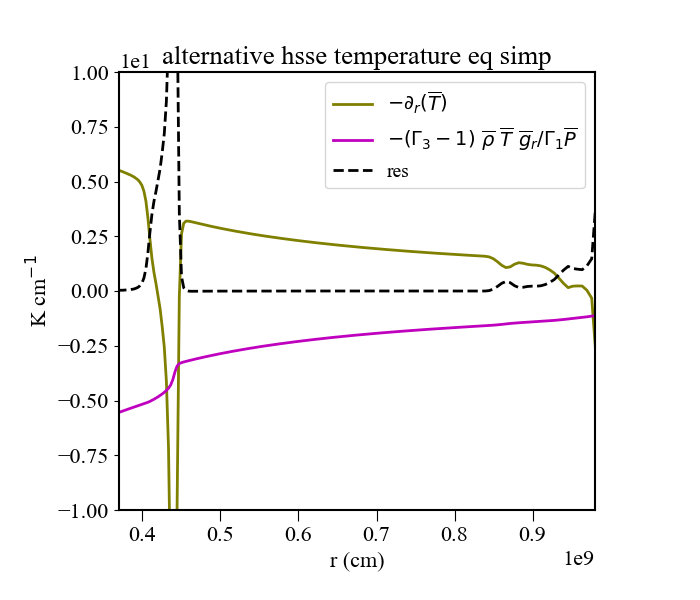
\includegraphics[width=6.3cm]{oblrez_hsse_temperature_eq_alternative_simplified.eps}
%  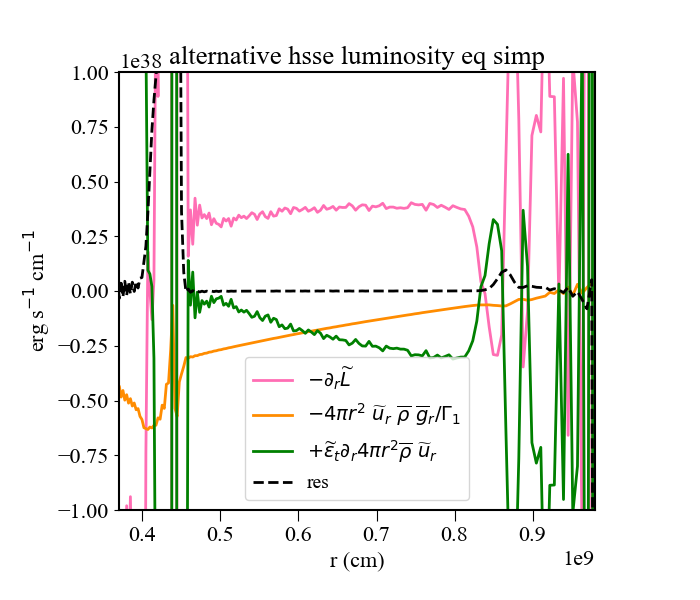
\includegraphics[width=6.3cm]{oblrez_hsse_luminosity_eq_alternative_simplified.eps}}

%\centerline{
%  \includegraphics[width=6.3cm]{oblrez_hsse_mean_Xtransport_ne20.eps}}
  
%\caption{Hydrodynamic stellar structure equations without MLT validated by 3D low-resolution oxygen burning convective shell simulation. Initial model is described more in detail in \citet{Mocak2018}.}
%\label{hsse:eq_simp}  
%\end{figure}

Partial results from our mean-field RANS analysis related mostly to turbulent kinetic energy and transport of some chemical elements based on oxygen burning shell in massive stars have been already published e.g. \citet{MeakinArnett2007,ArnettMeakin2009,Meakin2010,VialletMeakin2013,Mocak2018}.

In order to cover wider range of conditions present in stars like Schwarzschild and Ledoux stable/unstable regions, electron degeneracy and multiplicity of convection zones, I also plan to extend our library of ransX mean fields calculated during 3D high-resolution hydrodynamic simulations of: 

\begin{itemize}
\item single convection zone during core helium flash in low-mass stars with Ledoux unstable region at its bottom \citep{Mocak2008,Mocak2009,Mocak2011} (1+ year)
\item dual convection zone during core helium flash in metallicity free stars \citep{Mocak2010} (1+ year)
\item single convection zone resulting from core carbon flash in intermediate stars with Ledoux unstable region at its bottom \citep{Mocak2011} (1+ years)
\item O-Ne-C burning stellar interior in massive pre-supernova progenitor with multiple interacting convection zones \citep{Meakin2006} (3+ years)
%\item thermal pulse (model from Marcello)  
\end{itemize} 

The setups are already prepared in our MPI parallelized multi-species compressible fluid dynamics code PROMPI \citep{MeakinArnett2007}. Anticipated problems encompass computational time required to perform high-resolution 3D simulations, that may require 100k CPU hours for a single convective turnover timescale. In order to get statistically robust mean-fields from our framework, we need to simulate at least three such timescales per model after initial transient behaviour.

Besides general understading of the time-dependency, non-local and compressibility effects of turbulent convection in stars, these simulations will also serve as test beds for turbulence models inspired by work of \citet{rogers1989,lazeroms2013} and \citet{biferale2011}.

\section{Summary}

\begin{itemize}
\item publish comprehensive description and validation of the ransX framework in referred journal
\item extend our library of 3D hydrodynamic simulations with core helium flash, core carbon flash, dual core flash and O-Ne-C burning shell simulations (setups already prepared in our hydrodynamic code PROMPI)
\item develop turbulence models suitable for 1D stellar evolution calculations inspired by engineering turbulence literature with focus on turbulent composition flux, which in reactive flow controls nuclear reaction rates
\item make ransX a standard analysis tool in as many hydrodynamic codes as possible
\end{itemize}
  
\section{Intended Collaboration and Topic}

\begin{itemize}
\item Simon Campbell (Monash Centre for Astrophysics, Australia)
\begin{itemize}
\item 3D simulations of dual core flashes and nucleosynthesis in low-mass stars    
\end{itemize}  
\item Casey Meakin (Karagozian and Case, Inc., Glendale, California)
\begin{itemize}
\item turbulence modelling, ransX development, hydrodynamic stellar structure equations
\end{itemize}  
\item Dave Arnett (Steward Observatory, University of Arizona)
\begin{itemize}
\item turbulence modelling, hydrodynamic stellar structure equations
\end{itemize}   
\item Cyril Georgy (Geneva Observatory, University of Geneva, Switzerland)
\begin{itemize}
\item ransX development, hydrodynamic stellar structure equations
\end{itemize}    
\item Ewald Mueller (Max-Planck-Institut f\"ur Astrophysik, Germany)
\begin{itemize}
\item search for origin of gravitational wave signals during 3D hydrodynamic simulations of core-collapse supernovas using ransX framework 
\end{itemize} 
\end{itemize}
  
%\section{Definitions}

%\begin{align}                                                      
%  & \rho \ \ \mbox{density}                                           & & g_r  \ \ \mbox{radial gravitational acceleration} \nonumber \\
%  & m = \rho V = \rho \frac{4}{3} \pi r^3\ \ \mbox{mass}              & & M = \int \rho(r) dV \ \ \mbox{integrated mass} \nonumber \\  
%& T \ \ \mbox{temperature}                                          & & X_i \ \ \mbox{mass fraction)} \nonumber \\
%& P \ \ \mbox{pressure}                                             & & \epsilon_t \ \ \ \mbox{specific total energy} \nonumber \\ 
%& u_r, u_\theta, u_\phi \ \ \mbox{velocity components}                 & & f_i = \eht{\rho}\fht{X''_i u''_i} \ \ \mbox{composition flux}  \nonumber \\
%& {\bf u} = u (u_r, u_\theta, u_\phi) \ \ \mbox{velocity}               & &  d = \nabla \cdot {\bf u} \ \ \mbox{dilatation}    \nonumber \\              
%& \Gamma_1 = (d \ ln \ P/ d \ ln \ \rho)|_s                     & & \Gamma_2 / (\Gamma_2 -1) =  (d \ ln \ P/ d \ ln \ T)|_s \nonumber \\ 
%& \Gamma_3 -1 =  (d \ ln \ T/ d \ ln \ \rho)|_s                             & &  \nonumber 
%\end{align}

%add here also horizontal and statistical operator definitions, definition of X'' and u''r and the operators


\bibliography{referenc}

\end{document}


